\documentclass[a4paper]{article}
\usepackage{xunicode}
\usepackage{fontspec}
\usepackage{graphicx}
\usepackage{kpfonts}
\usepackage[T1]{fontenc}


\renewcommand*{\familydefault}{\sfdefault}

\renewcommand{\nobreakspace}{\nobreak\ }

\begin{document}
	\begin{titlepage}
		\begin{center}
		
\includegraphics{logo_fac.png}\\[3.0cm]
		{\Huge ALMA' TWE}\\[0.5cm]
		{\huge\itshape How to loose time with Open ESB}\\[3.0cm]
		\end{center}
		
		\begin{minipage}{0.4\textwidth}
		\begin{flushleft}
			\emph{Authors:}\\[0.1cm]
			Julien \textsc{Durillon}\\
			Alexandre \textsc{Garnier}
		\end{flushleft}
		\end{minipage}
		\begin{minipage}{0.4\textwidth}
		\begin{flushright}
			\emph{Date :}\\[0.1cm]
			\today
		\end{flushright}
		\end{minipage}
		
	\end{titlepage}

	\tableofcontents\clearpage

	\section*{Introduction}
	\addcontentsline{toc}{section}{Introduction}

	\section{First approach}
	
		\subsection{Main process}
		
		
			The process for using the ALMA TWE service is the following: first, a user look up for events matching criteria (figure \ref{fig:lookup}), then book the week-end for the choosen event (figure \ref{fig:mainprocrequest}): travel, hostel, restaurant.
			
			%% Ici figures lookup et mainprocrequest
			\begin{figure}[htp]
				\centering
				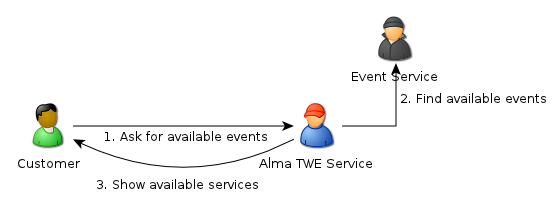
\includegraphics[width=\textwidth]{lookupprocess.png}
				\caption{Event lookup process}
				\label{fig:lookup}
			\end{figure}
			
			\begin{figure}[htp]
				\centering
				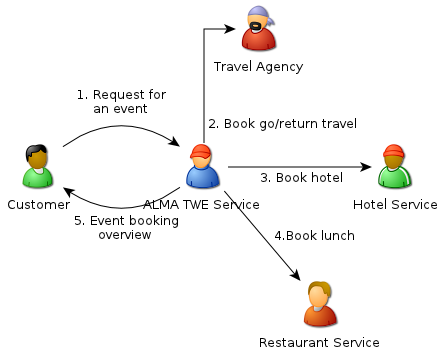
\includegraphics[width=\textwidth]{bookingprocess.png}
				\caption{Event booking process}
				\label{fig:mainprocrequest}
			\end{figure}
			
			
			
		\subsection{Requesting a week-end package}
		
			When the main controller receives a week-end request for an event, it first books the round-up travel, then the hostel for the night, and then the restaurant for the evening lunch before the event. The figure \ref{fig:bookingprocess} describes the whole booking process and the exchanged data.
			
			\begin{figure}[htp]
				\centering
				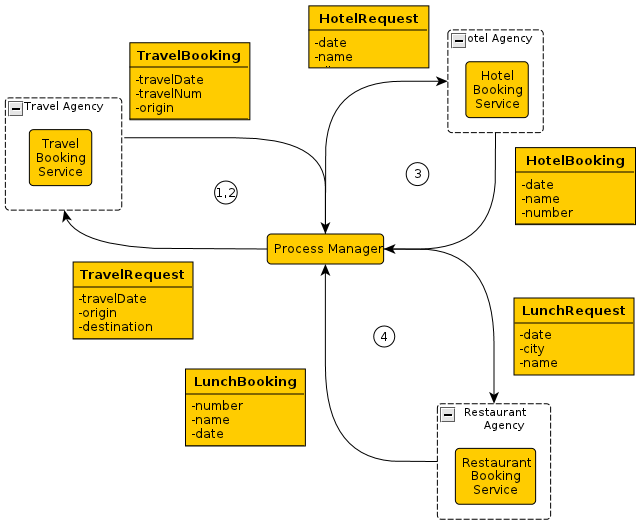
\includegraphics[width=\textwidth]{processmanager.png}
				\caption{Event booking process: with data}
				\label{fig:bookingprocess}
			\end{figure}
			
	
	
	\section{Services}
	
		There are 4 services in the ALMA TWE: Hostel, Restaurant, Event and Travel. All theses services are composed by a 5th one : CASATWE. This one furnishes a wsdl, that will be used by the user interface.
	
	
	\section{Databases}
	
		\subsection{Database schemes}
		
		The services need databases in order to store and retrieve booking informations. We need then a table for each service that stores available choices, and a table for table for each service that stores booking. The figure \ref{fig:globaldb} describes the differents tables used by the services. Two tables of differents services have no connection between them.
		
		\begin{figure}[htp]
			\centering
			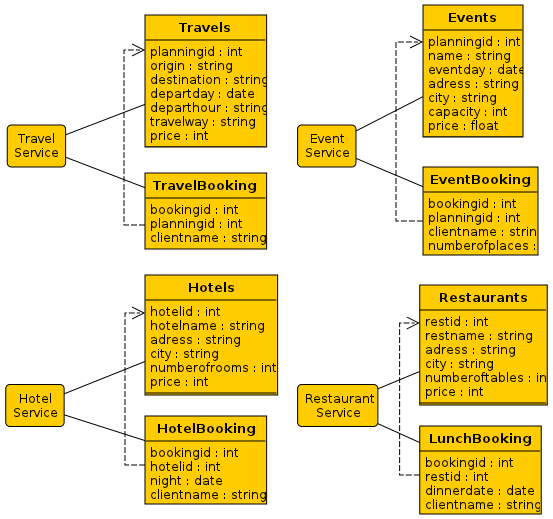
\includegraphics[width=\textwidth]{database.png}
			\caption{Tables for each services}
			\label{fig:globaldb}
		\end{figure}
	
	
	
	
	
	\section{User interfaces}
	
	\section*{Conclusion}
	\addcontentsline{toc}{section}{Conclusion}



\end{document}